\chapter{Introduction} \label{chap:intro}
\renewcommand{\tabdir}{chapters/intro/tab}
\renewcommand{\figdir}{chapters/intro/fig}

\section{The \software{echse} simulation environment} \label{sec:intro_idea}

The idea of a \emph{simulation environment}\index{simulation environment}\index{modeling framework|see{simulation environment}}\index{generic model|see{simulation environment}} is to provide a tool which can be used to simulate different systems and/or processes in a single unified software environment. Terms sometimes used more or less synonymously are \emph{modeling framework}, \emph{generic model} or \emph{open structure} model. Examples of existing modeling frameworks in the field of earth and environmental sciences include the \emph{Object Modeling System} \citep{Ahuja2005} and the \emph{Earth System Modeling Framework} \citep{Hill2004}. Examples from the field of water quality modeling include, for example, \emph{AQUASIM} \citep{Reichert1998}, the biogeochemical reactions network simulator BRNS \citep{Regnier2002, Thullner2005}, and the \emph{ECO Lab} software \citep{DHI2006}.

The benefit of a modeling framework usually emerges in situations, where
\begin{itemize}
  \item new models have to be developed in short time.
  \item a preliminary model has to be build and later improvement (possibly by different staff) is planned.
  \item alternative model structures are to be compared (to find an optimum structure or to learn about structural uncertainty).
  \item different people are involved in collaborative model development.
  \item a larger number of individual models must be used and a common (user) interface for all models is required (in operational forecasting, for example).
\end{itemize}

A basic characteristics of a modeling framework is the flexibility to simulate \emph{objects} of different \emph{classes} \footnote{An approximate synonym is \emph{types}.}. Typically, the features of a class, which include \emph{data} and \emph{methods} \footnote{An approximate synonym is \emph{functions}.} are declared/defined by the developer of a specific model for a specific purpose. In contrast to that, the generic core of the modeling framework represents the static part of the software, providing the basic infrastructure for all models (\figref{fig:intro-modelingFramework}).

\begin{figure}
  \centering
  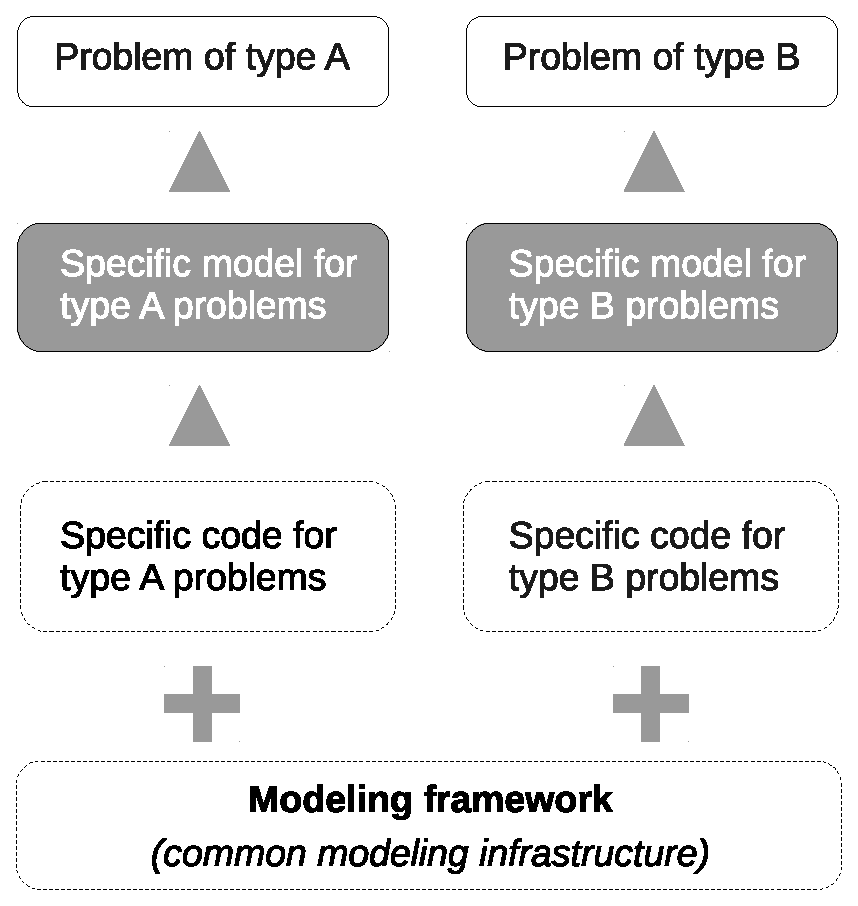
\includegraphics[width=0.9\columnwidth]{\figdir/modelingFramework.eps}
  \caption{Basic idea of a modeling framework. \label{fig:intro-modelingFramework}}
\end{figure}

The \software{echse}\index{\software{echse}} is intended to be a lightweight, simple to use modeling framework, being applicable to many (but not all) simulation problems, arising in the field of (eco)-hydrology. Details on potentials and limits are summarized in \secref{sec:intro_potentials-limits} and discussed in more detail in \chapref{chap:concept}.

It is important to understand that the \software{echse} simulation environment actually consists of two parts:
\begin{description}
  \item [The generic model core] This is a collection of source files. These files provide the common modeling intrastructure shown at the bottom of \figref{fig:intro-modelingFramework}.
  \item [The code generator] This is a software (currently implemented in R) to generate a large part of the \emph{application-specific} source code from basic information provided by the model developer. The generated source code is guaranteed to be compatible with the source code of the generic model core.
\end{description}

In order to create a specific model (grey boxes in \figref{fig:intro-modelingFramework}), the model developer finally has to complement the generated source code by implementing a set of methods (functions) with a simple, well defined interface. Only at this step, source code has to be written manually.

\section{Potential uses and limits} \label{sec:intro_potentials-limits}

Since the potential model applications in the field of eco-hydrology are so diverse, there is (and there cannot be) a modeling framework which is equally suitable for all those applications. Consequently, a 'good' modeling framework is usually one that is specialized on a certain range of applications (as opposed to a 'normal' model, that is specialized on a certain application alone).

The \software{echse} has been developed in the context of hydrological catchment modeling and water quality modeling. Therefore, this modeling framework is particularly specialized on
\begin{itemize}
  \item the simulation of a collection of objects representing instances of different classes (\eg{} catchments, river sections, lakes, etc.).
  \item the simulation of object interactions that are mostly of the \emph{feed-forward} type, \ie{} the simulated flow of mass, energy, or information is mostly unidirectional. \emph{Feedbacks}, \ie{} two-way interations between objects, may also be simulated but there are currently limitations with respect to the accuracy of results.
\end{itemize}

The current version of the \software{echse} is \emph{not} recommended for building models that
\begin{itemize}
  \item are dominated by feedback interactions between the simulated objects. That is, for example, the case in ground water or hydrodynamic modeling, where \emph{partial differential equations} (PDE) have to be solved. The concept of the \software{echse} currently does not support high-accuracy solutions of PDE.
  \item consist of a single object only. Simualting a single object is not a practical problem, but the use of other modeling tools may simply be more efficient.
\end{itemize}

\section{Required user skills} \label{sec:intro_skills}

\subsection{Use of existing models} \label{sec:intro_skills-use}

The skills required for using an existing model built with the \software{echse} are the same as for any other dynamic system model. You basically need to
\begin{itemize}
  \item understand the characteristics of the implemented classes (from a documentation of the specific model).
  \item know which input files are required (see \chapref{chap:input}).
  \item be able to create all input files. This can be done manually (for small projects only), by writing skripts (for example using R, Matlab, Python, etc.), and/or by using other programs such as spreadsheet software, geographical information systems, or data bases.
  \item understand the limits of the implemented model with respect to your specific application.
\end{itemize}

\subsection{Development of models} \label{sec:intro_skills-dev}

As with all modeling frameworks, the \software{echse} aims at reducing the effort for building new models and for changing/extending existing ones. Thus, you don't need to be a professional code writer. However, to successfully create or modify models, you should
\begin{itemize}
  \item understand the meaning of the terms 'class' and 'object' (see any introduction on object-oriented programming),
  \item know the different features of a class supported by \software{echse} and understand the meaning of the classes' 'simulate' methods (see \chapref{chap:concept}),
  \item have basic knowledge of ordinary differential equations and their use in the simulation of dynamic systems,
  \item be able to program simple algorithms in any language,
  \item be willing to get familiar with the most basic elements of C++ (basic data types, operators, and flow-control) or find someone who will translate (or wrap) your code if written in another language.
\end{itemize}
